\chapter{Entropia e energia de Gibbs de reação}\label{ch:b2:reaction-free-energy}

Uma bolsa de gelo instantâneo, dessas usadas no esporte, contém um saco de
água e algumas colheres de nitrato de amônio. Basta apertá-la: o saco
interno se rompe, o sal se dissolve e, em segundos, a bolsa está fria o
bastante para aliviar um tornozelo torcido. A dissolução absorve calor ---
ela é \omterm{def:b2:reaction-enthalpy:exothermic}{endotérmica} --- e, no entanto, ocorre sozinha, até o fim. A entalpia
do capítulo anterior não pode ser toda a história: uma reação não segue
apenas ``ladeira abaixo em calor''. A grandeza que falta é a entropia, que
a segunda lei da termodinâmica, vista na física, torna o juiz de toda
transformação espontânea. Este capítulo tabela entropias, calcula a
entropia de uma reação e combina entalpia e entropia em uma única função,
a \omterm{def:b2:reaction-free-energy:gibbs-energy}{energia de Gibbs}, cuja derivada de reação decide o sentido de toda
reação a temperatura e pressão fixas.

\begin{recall}
Da física: a segunda lei. Todo sistema tem uma função de estado, sua
entropia $S$ (extensiva); em uma transformação de um sistema fechado, $\dd S =
\delta Q/T_{\text{ext}} + \delta S_{\text{c}}$, em que a entropia criada
$\delta S_{\text{c}}$ é nula para uma transformação reversível e positiva
nos demais casos; para um sistema fechado de composição fixa, $\dd U = T\dd S -
p\dd V$. \Cref{ch:b2:reaction-enthalpy}: \omterm{def:b2:reaction-enthalpy:reaction-quantity}{grandezas de reação} $\Delta_r X =
(\partial X/\partial\xi)_{T,p}$ e \omterm{def:b2:reaction-enthalpy:standard-reaction-enthalpy}{entalpias padrão de reação}. O volume do
1.º ano enunciou, como leis ``que decorrem da segunda lei'', que uma
reação evolui até $Q = K^\circ$; este capítulo e os dois seguintes as
demonstram.
\end{recall}

\begin{omfigure}
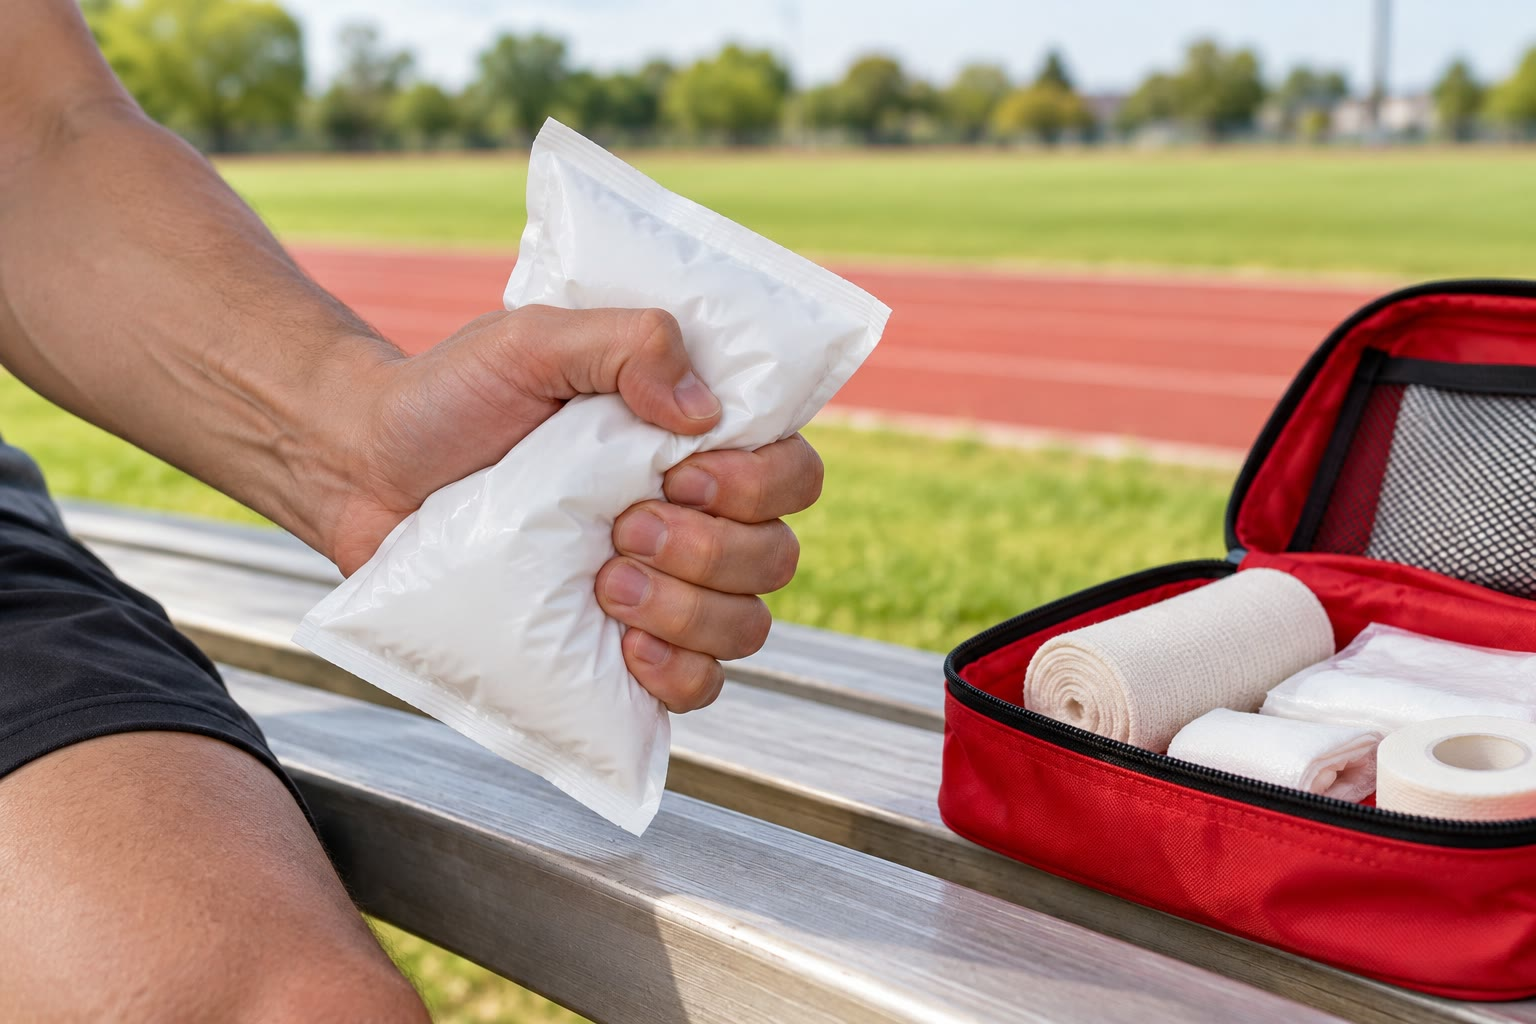
\includegraphics[width=0.55\linewidth]{images/book3/ai/b2-02-cold-pack.jpg}

{\small Uma bolsa de gelo instantâneo: quando o saco interno se rompe, o
nitrato de amônio se dissolve na água e a bolsa esfria. A dissolução é
\omterm{def:b2:reaction-enthalpy:exothermic}{endotérmica} e espontânea; sua entropia explica por quê (\cref{ex:b2:reaction-free-energy:cold-pack}).}
\end{omfigure}

\section{Entropias padrão e terceira lei}

Ao contrário da entalpia, a entropia tem um zero natural.

\begin{theorem}[Terceira lei da termodinâmica]\label{thm:b2:reaction-free-energy:third-law}
A entropia de um cristal puro e perfeitamente ordenado tende a zero quando
sua temperatura tende a \qty{0}{K}.
\end{theorem}
\admitted

\begin{remark}[De onde vem o zero]\label{rem:b2:reaction-free-energy:third-law}
Walther Nernst enunciou em 1906 que as \omterm{def:b2:reaction-free-energy:reaction-entropy}{entropias de reação} entre fases
condensadas se anulam quando $T \to 0$; Max Planck a tornou mais precisa,
no enunciado acima. Sua origem é estatística: a entropia conta os arranjos
microscópicos compatíveis com o estado de um sistema, e um cristal perfeito
a \qty{0}{K} tem um só. A contagem é feita no volume do 3.º ano,
com as funções de partição.
\end{remark}

\begin{definition}[Entropia molar padrão]\label{def:b2:reaction-free-energy:standard-entropy}
A \emph{entropia molar padrão}\index{entropia molar padrao@entropia molar padrão}
$S^\circ_m(T)$ de uma substância é a entropia de um mol dela em seu
estado padrão à temperatura $T$, sendo o zero o da terceira lei.
Ao contrário de $\Delta_f H^\circ$, é uma grandeza absoluta, positiva para
toda substância, inclusive os elementos.
\end{definition}

\begin{proposition}[Entropia absoluta a partir das capacidades caloríficas]\label{prop:b2:reaction-free-energy:absolute-entropy}
Aquecendo uma substância à pressão constante $p^\circ$ de \qty{0}{K} a $T$,
\[
  S^\circ_m(T) = \int_0^T\frac{C^\circ_{p,m}(T')}{T'}\,\dd T' +
  \sum_{\text{transições}}\frac{\Delta_{\text{trs}}H^\circ}{T_{\text{trs}}} ,
\]
sendo a integral tomada, em cada fase, sobre seu intervalo de temperatura.
\end{proposition}

\begin{proof}
Aqueça a substância de modo reversível a pressão constante: $\delta S_{\text{c}} =
0$ e $\delta Q = \dd H = C_p\,\dd T$, logo $\dd S = C_p\,\dd T/T$. Em uma
transição (fusão, ebulição), a temperatura fica em $T_{\text{trs}}$
enquanto o calor $\Delta_{\text{trs}}H$ é recebido de modo reversível: a
entropia salta de $\Delta_{\text{trs}}H/T_{\text{trs}}$. Some as parcelas a
partir do zero da terceira lei.
\end{proof}

\begin{omfigure}
\begin{tikzpicture}
\begin{axis}[
  width=0.8\linewidth, height=6.2cm, xmin=0, xmax=1500, ymin=0, ymax=210,
  axis x line=bottom, axis y line=left, xlabel={$T$ (K)},
  ylabel={$S^\circ_m$ do zinco (\unit{J/(K.mol)})},
  xtick={0,250,500,750,1000,1250,1500},
  tick label style={font=\small}, label style={font=\small}, clip=false]
\addplot[omDef, very thick, smooth] table[x=T, y=S] {figdata/out/bachelor-2-standard-entropy-solid.dat};
\addplot[omProp, very thick] table[x=T, y=S] {figdata/out/bachelor-2-standard-entropy-liquid.dat};
\addplot[omThm, very thick] table[x=T, y=S] {figdata/out/bachelor-2-standard-entropy-gas.dat};
\draw[densely dashed, gray] (axis cs:692.73,64.6) -- (axis cs:692.73,75.2);
\draw[densely dashed, gray] (axis cs:1180.2,91.9) -- (axis cs:1180.2,189.6);
\node[omDef, font=\small, anchor=south east] at (axis cs:600,60) {sólido};
\node[omProp, font=\small, anchor=north west] at (axis cs:850,78) {líquido};
\node[omThm, font=\small, anchor=south] at (axis cs:1350,192) {gás};
\node[font=\scriptsize, anchor=west, align=left] at (axis cs:700,110) {fusão, $+10.6$\\ a \qty{692.7}{K}};
\node[font=\scriptsize, anchor=east, align=right] at (axis cs:1170,150) {ebulição,\\ $+97.7$ a\\ \qty{1180.2}{K}};
\end{axis}
\end{tikzpicture}

{\small \omterm{def:b2:reaction-free-energy:standard-entropy}{Entropia molar padrão} do zinco a partir do zero da terceira lei. Ela
cresce com a temperatura à medida que o metal armazena calor, depois salta
no ponto de fusão de $\Delta_{\text{fus}}H/T_{\text{fus}}$ e, muito mais,
no ponto de ebulição de $\Delta_{\text{vap}}H/T_b$: um gás é muito mais
desordenado que um líquido.}
% ledger: s0T:Zn_crl.0, s0T:Zn_crl.298.15, s0T:Zn_cr.692, s0T:Zn_l.692, s0T:Zn_l.1180, s0T:Zn_g.1180, hT:Zn_cr.692, hT:Zn_l.692, hT:Zn_l.1180, hT:Zn_g.1180, dfh:Zn_g (curve in figdata/bachelor-2/standard-entropy.py)
\end{omfigure}

A figura dá ordens de grandeza que vale a pena guardar. À temperatura
ambiente, um metal ou um cristal duro tem algumas dezenas de
\unit{J/(K.mol)}, um líquido cerca de cem, um gás de cem a trezentos; a
fusão acrescenta pouco, a ebulição acrescenta muito. As \omterm{def:b2:reaction-free-energy:standard-entropy}{entropias molares
padrão} usadas neste volume são tabeladas com as entalpias de formação.

\section{Entropia de reação}

\begin{definition}[Entropia de reação]\label{def:b2:reaction-free-energy:reaction-entropy}
A \emph{entropia de reação}\index{entropia de reacao@entropia de reação} é $\Delta_r S =
(\partial S/\partial\xi)_{T,p}$, e a \emph{entropia padrão de
reação}\index{entropia padrao de reacao@entropia padrão de reação} é $\Delta_r S^\circ(T) =
\sum_i\nu_iS^\circ_{m,i}(T)$, em \unit{J/(K.mol)}.
\end{definition}

Como as entropias padrão são absolutas, não é preciso nenhuma reação de
formação: os elementos entram com suas próprias entropias.

\begin{example}[Três entropias de reação]\label{ex:b2:reaction-free-energy:entropies}
A \qty{298.15}{K}:
\begin{itemize}
  \item \ce{CaCO3(s) -> CaO(s) + CO2(g)}: $\Delta_r S^\circ = 39.75 + 213.79 -
        92.9 = \qty{+160.6}{J/(K.mol)}$, um gás formado a partir de um sólido;
  \item \ce{N2(g) + 3H2(g) -> 2NH3(g)}: $\Delta_r S^\circ = 2(192.77) -
        191.61 - 3(130.68) = \qty{-198.1}{J/(K.mol)}$, quatro moléculas de gás
        que se tornam duas;
  \item \ce{N2O4(g) -> 2NO2(g)}: $\Delta_r S^\circ = 2(240.03) - 304.38 =
        \qty{+175.7}{J/(K.mol)}$.
\end{itemize}
% ledger: s0:CaCO3_cr, s0:CaO_cr, s0:CO2_g, s0:N2_g, s0:H2_g, s0:NH3_g, s0:N2O4_g, s0:NO2_g (computed in figdata/bachelor-2/thermo-data.py)
\end{example}

\begin{proposition}[O sinal de uma entropia de reação]\label{prop:b2:reaction-free-energy:sign-rule}
Quando participam gases, o sinal de $\Delta_r S^\circ$ é, em geral, o de
$\Delta\nu_{\text{gás}} = \sum_{\text{gases}}\nu_i$, e sua magnitude é de cerca de
\qty{100}{} a \qty{200}{J/(K.mol)} por mol de gás formado ou consumido. Quando
$\Delta\nu_{\text{gás}} = 0$, ou não há gás envolvido, $\Delta_r S^\circ$ é
pequena e seu sinal precisa ser calculado.
\end{proposition}

\begin{proof}[Justificativa]
A entropia molar de um gás a \qty{298}{K} fica entre 130 e
\qty{300}{J/(K.mol)}, a de um sólido ou de um líquido em algumas dezenas:
formar ou consumir um mol de gás domina todas as outras contribuições. É
uma regra prática, não um teorema: a dissolução de um sal, sem gás, ainda
pode mudar a entropia de uma centena de \unit{J/(K.mol)}.
\end{proof}

\begin{method}[Prever o sinal de $\Delta_r S^\circ$]\label{met:b2:reaction-free-energy:entropy-sign}
\begin{enumerate}
  \item Calcule $\Delta\nu_{\text{gás}}$: se não for nulo, ele dá o
        sinal.
  \item Caso contrário, compare a ordem dos estados: dissolver um cristal,
        fundir, partir uma molécula em dois pedaços aumentam a entropia;
        precipitar, solidificar, juntar duas moléculas em uma a diminuem.
  \item Quando a decisão importa, calcule $\sum_i\nu_iS^\circ_{m,i}$.
\end{enumerate}
\end{method}

O volume do 1.º ano encontrou uma consequência disso: uma eliminação forma
mais moléculas que uma substituição com os mesmos reagentes (o alceno, o
grupo de saída e a base protonada, contra o produto de substituição e o
grupo de saída). Sua \omterm{def:b2:reaction-free-energy:reaction-entropy}{entropia de reação} é maior, e o termo entrópico, que
cresce com a temperatura, como mostra a próxima seção, é a razão pela qual
o aquecimento favorece a eliminação em relação à substituição.

\section{A energia de Gibbs}

\begin{definition}[Energia de Gibbs]\label{def:b2:reaction-free-energy:gibbs-energy}
A \emph{energia de Gibbs}\index{energia de Gibbs} (ou entalpia livre) de um sistema
é a função de estado $G = H - TS$, extensiva, em joules.
\end{definition}

\begin{definition}[Energia de Gibbs de reação]\label{def:b2:reaction-free-energy:reaction-gibbs}
A \emph{energia de Gibbs de reação}\index{energia de Gibbs de reacao@energia de Gibbs de reação} é $\Delta_r G
= (\partial G/\partial\xi)_{T,p}$, e a \emph{energia de Gibbs padrão de
reação}\index{energia de Gibbs padrao de reacao@energia de Gibbs padrão de reação} é $\Delta_r G^\circ(T) =
\sum_i\nu_iG^\circ_{m,i}(T)$, ambas em \unit{kJ/mol}.
\end{definition}

\begin{proposition}[Termos entálpico e entrópico]\label{prop:b2:reaction-free-energy:g-h-s}
$\Delta_r G = \Delta_r H - T\Delta_r S$, e $\Delta_r G^\circ = \Delta_r
H^\circ - T\Delta_r S^\circ$.
\end{proposition}

\begin{proof}
Derive $G = H - TS$ em relação a $\xi$ a $T$ e $p$ fixos: $T$
é uma constante na derivação.
\end{proof}

\begin{proposition}[Diferencial de $G$ para um sistema em reação]\label{prop:b2:reaction-free-energy:dG}
Para um sistema fechado no qual ocorre uma reação, a $T$ e
$p$ uniformes,
\[
  \dd G = V\,\dd p - S\,\dd T + \Delta_r G\,\dd\xi .
\]
\end{proposition}

\begin{proof}
$G(T, p, \xi)$ tem a diferencial exata $\dd G = (\partial G/\partial
T)_{p,\xi}\dd T + (\partial G/\partial p)_{T,\xi}\dd p + \Delta_r G\,\dd\xi$.
As duas primeiras derivadas parciais são tomadas a composição fixa: são
as de um sistema fechado de composição fixa, para o qual a física dá
$\dd U = T\dd S - p\dd V$, de modo que $\dd G = \dd U + p\dd V + V\dd p - T\dd S
- S\dd T = V\dd p - S\dd T$. Logo $(\partial G/\partial T)_{p,\xi} = -S$
e $(\partial G/\partial p)_{T,\xi} = V$.
\end{proof}

\section{O critério de evolução}

\begin{theorem}[Critério de evolução]\label{thm:b2:reaction-free-energy:evolution}
Em um sistema fechado mantido a temperatura e pressão constantes, que não
troca outro trabalho além do das forças de pressão, uma reação só pode
avançar no sentido que torna
\[
  \Delta_r G\,\dd\xi \leq 0 ,
\]
com igualdade no equilíbrio. Se $\Delta_r G < 0$, a reação avança no
sentido direto; se $\Delta_r G > 0$, no sentido inverso; e o sistema está em
equilíbrio quando $\Delta_r G = 0$.
\end{theorem}

\begin{proof}
Considere uma transformação infinitesimal a $T$ e $p$ uniformes, iguais às da
vizinhança. A primeira lei, apenas com trabalho de pressão, dá $\dd U = \delta Q
- p\dd V$; a segunda dá $\delta Q = T\dd S - T\delta S_{\text{c}}$. Então
\[
  \dd G = \dd U + p\dd V + V\dd p - T\dd S - S\dd T = -T\,\delta
  S_{\text{c}} + V\dd p - S\dd T .
\]
Comparando com a \cref{prop:b2:reaction-free-energy:dG}, a $T$ e $p$ fixos:
$\Delta_r G\,\dd\xi = -T\,\delta S_{\text{c}}$. Como $\delta S_{\text{c}}
\geq 0$, $\Delta_r G\,\dd\xi \leq 0$, e $\delta S_{\text{c}} = 0$ (uma
transformação reversível, de equilíbrio) exige $\Delta_r G = 0$.
\end{proof}

\begin{remark}[O que o critério diz, e o que não diz]\label{rem:b2:reaction-free-energy:criterion}
A entropia criada por uma reação a $T$ e $p$ constantes é $-\Delta_r G\,
\dd\xi/T$: a \omterm{def:b2:reaction-free-energy:gibbs-energy}{energia de Gibbs} é a segunda lei, restrita às condições
do laboratório e escrita com grandezas do próprio sistema. Ela diz
em que sentido uma reação pode ir, nunca com que velocidade: o diamante,
cuja conversão em grafita tem $\Delta_r G^\circ < 0$, dura para sempre em
um anel. E ela supõe que não há outro trabalho: uma pilha que fornece
trabalho elétrico, ou um eletrolisador que o recebe, obedece a um critério
modificado (\cref{ch:b2:cell-thermodynamics}).
\end{remark}

\begin{definition}[Exergônica e endergônica]\label{def:b2:reaction-free-energy:exergonic}
Uma reação é \emph{exergônica}\index{exergonica@exergônica} em um dado estado quando
$\Delta_r G < 0$ e \emph{endergônica}\index{endergonica@endergônica} quando $\Delta_r G >
0$. Com todas as espécies em seu estado padrão, essas palavras se aplicam ao
sinal de $\Delta_r G^\circ$.
\end{definition}

O critério usa $\Delta_r G$, o valor no estado real do
sistema; $\Delta_r G^\circ$ se refere a todas as espécies em seu estado
padrão, que raramente é o estado de uma mistura real. A ligação entre os
dois, pela composição, é o assunto do \cref{ch:b2:chemical-potential}, e
dá a lei $Q = K^\circ$ do 1.º ano no \cref{ch:b2:equilibrium-shifts}. Para
reações entre sólidos e líquidos puros, e gases a \qty{1}{bar}, os
dois coincidem.

\begin{example}[A bolsa de gelo instantâneo]\label{ex:b2:reaction-free-energy:cold-pack}
Para \ce{NH4NO3(s) -> NH4+(aq) + NO3-(aq)} a \qty{298.15}{K}, nos estados
padrão: $\Delta_r H^\circ = -339.87 + 365.56 = \qty{+25.69}{kJ/mol}$ e
$\Delta_r S^\circ = 259.8 - 151.08 = \qty{+108.7}{J/(K.mol)}$, logo
$\Delta_r G^\circ = 25.69 - 298.15 \times 0.1087 = \qty{-6.7}{kJ/mol}$: a
dissolução é \omterm{def:b2:reaction-enthalpy:exothermic}{endotérmica} e \omterm{def:b2:reaction-free-energy:exergonic}{exergônica}. Os íons, livres na água, são
mais desordenados que no cristal, e o termo entrópico $T\Delta_r
S^\circ = \qty{32.4}{kJ/mol}$ supera o custo entálpico.
% ledger: dfh:NH4NO3_cr, s0:NH4NO3_cr, dfh:NH4NO3_ai, s0:NH4NO3_ai (computed in figdata/bachelor-2/thermo-data.py)
\end{example}

\begin{history}[Josiah Willard Gibbs]
\begin{minipage}[t]{0.2\linewidth}\vspace{0pt}
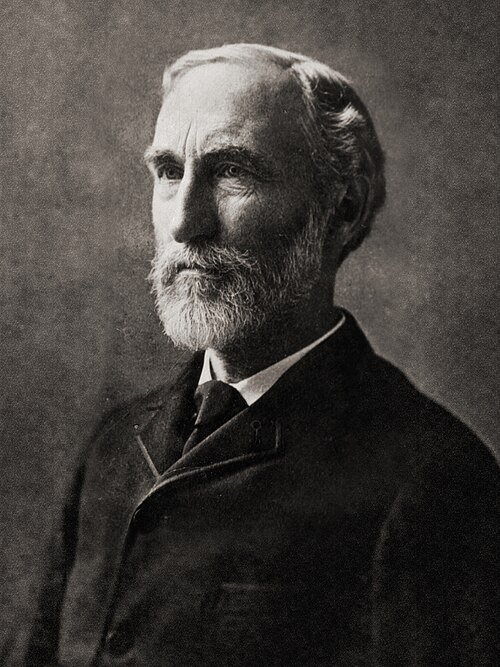
\includegraphics[width=\linewidth]{images/book3/gibbs.jpg}
\end{minipage}\hfill
\begin{minipage}[t]{0.76\linewidth}\vspace{0pt}
Josiah Willard Gibbs (1839--1903), professor de física matemática em
Yale, publicou entre 1876 e 1878 \emph{On the Equilibrium of
Heterogeneous Substances}, umas trezentas páginas nas atas de uma pequena
academia, nas quais aparecem a energia livre, o potencial químico e a
regra das fases dos próximos capítulos. Poucos químicos o leram antes
de sua tradução, na década de 1890. (Fotografia: domínio público,
Wikimedia Commons.)
\end{minipage}
\end{history}

\section{Energias de Gibbs padrão de reação e temperatura}

\begin{definition}[Aproximação de Ellingham]\label{def:b2:reaction-free-energy:ellingham-approximation}
A \emph{aproximação de Ellingham}\index{aproximacao de Ellingham@aproximação de Ellingham} trata
$\Delta_r H^\circ$ e $\Delta_r S^\circ$ como independentes da temperatura
em um intervalo que não contém mudança de estado. Então $\Delta_r G^\circ(T)
= \Delta_r H^\circ - T\Delta_r S^\circ$ é uma reta em $T$, de inclinação
$-\Delta_r S^\circ$.
\end{definition}

\begin{proposition}[Derivadas em relação à temperatura]\label{prop:b2:reaction-free-energy:gibbs-helmholtz}
\[
  \frac{\dd\Delta_r G^\circ}{\dd T} = -\Delta_r S^\circ, \qquad
  \frac{\dd}{\dd T}\!\left(\frac{\Delta_r G^\circ}{T}\right) =
  -\frac{\Delta_r H^\circ}{T^2}\ \ \text{(Gibbs--Helmholtz)}, \qquad
  \frac{\dd\Delta_r S^\circ}{\dd T} = \frac{\Delta_r C^\circ_p}{T}.
\]
Em particular, a \omterm{def:b2:reaction-free-energy:ellingham-approximation}{aproximação de Ellingham} vale quando $\Delta_r C^\circ_p$
é pequena.
\end{proposition}

\begin{proof}
Com todas as espécies em seu estado padrão, $G^\circ(T, \xi)$ tem $(\partial
G^\circ/\partial T)_\xi = -S^\circ$ (\cref{prop:b2:reaction-free-energy:dG}).
Pelo teorema de Schwarz,
\[
  \frac{\dd\Delta_r G^\circ}{\dd T} = \partial_\xi\partial_T G^\circ =
  -\partial_\xi S^\circ = -\Delta_r S^\circ .
\] Então $\frac{\dd}{\dd
T}(\Delta_r G^\circ/T) = \frac{-T\Delta_r S^\circ - \Delta_r G^\circ}{T^2} =
-\frac{\Delta_r H^\circ}{T^2}$. Por fim, $\dd S^\circ_m = C^\circ_{p,m}\,\dd
T/T$ para cada espécie (\cref{prop:b2:reaction-free-energy:absolute-entropy}),
e a mesma combinação dá a última relação. Se $\Delta_r C^\circ_p$ é
pequena, $\Delta_r H^\circ$ (Kirchhoff) e $\Delta_r S^\circ$ quase não variam.
\end{proof}

\begin{definition}[Temperatura de inversão]\label{def:b2:reaction-free-energy:inversion-temperature}
Quando $\Delta_r H^\circ$ e $\Delta_r S^\circ$ têm o mesmo sinal, a
\emph{temperatura de inversão}\index{temperatura de inversao@temperatura de inversão} da reação é
a temperatura na qual $\Delta_r G^\circ$ muda de sinal; na \omterm{def:b2:reaction-free-energy:ellingham-approximation}{aproximação de
Ellingham}, $T_i = \Delta_r H^\circ/\Delta_r S^\circ$.
\end{definition}

\begin{omfigure}
\begin{tikzpicture}
\begin{axis}[
  width=0.72\linewidth, height=5.6cm, xmin=0, xmax=1600, ymin=0, ymax=260,
  axis x line=bottom, axis y line=left, xlabel={$T$ (K)}, ylabel={\unit{kJ/mol}},
  tick label style={font=\small}, label style={font=\small}, clip=false]
\addplot[omThm, very thick] table[x=T, y=DrH] {figdata/out/bachelor-2-thermo-data-calcite.dat};
\addplot[omDef, very thick] table[x=T, y=TDrS] {figdata/out/bachelor-2-thermo-data-calcite.dat};
\node[omThm, anchor=south west, font=\small] at (axis cs:60,180) {$\Delta_r H^\circ = 178.3$};
\node[omDef, anchor=west, font=\small] at (axis cs:1600,257) {$T\Delta_r S^\circ$};
\draw[dotted] (axis cs:1110,0) -- (axis cs:1110,178.3);
\node[anchor=south west, font=\small] at (axis cs:1120,8) {$T_i = \qty{1110}{K}$};
\node[font=\scriptsize, align=center] at (axis cs:600,140) {$\Delta_r G^\circ > 0$:\\ calcita\\ estável};
\node[font=\scriptsize, align=center] at (axis cs:1470,206) {$\Delta_r G^\circ < 0$};
\end{axis}
\end{tikzpicture}

{\small Os termos entálpico e entrópico de \ce{CaCO3(s) -> CaO(s) + CO2(g)}
na \omterm{def:b2:reaction-free-energy:ellingham-approximation}{aproximação de Ellingham}. Abaixo da \omterm{def:b2:reaction-free-energy:inversion-temperature}{temperatura de inversão}, o custo
entálpico vence e o calcário é estável sob \qty{1}{bar} de dióxido de
carbono; acima dela, o termo entrópico vence e o calcário se decompõe.}
% ledger: dfh:CaCO3_cr, dfh:CaO_cr, dfh:CO2, s0:CaCO3_cr, s0:CaO_cr, s0:CO2_g (computed in figdata/bachelor-2/thermo-data.py)
\end{omfigure}

\begin{omfigure}
\begin{tikzpicture}[font=\small]
  \draw[thick] (0,0) rectangle (8,4);
  \draw[thick] (4,0) -- (4,4) (0,2) -- (8,2);
  \node[above] at (2,4) {$\Delta_r H^\circ < 0$};
  \node[above] at (6,4) {$\Delta_r H^\circ > 0$};
  \node[left] at (0,3) {$\Delta_r S^\circ > 0$};
  \node[left] at (0,1) {$\Delta_r S^\circ < 0$};
  \node[align=center, omDef] at (2,3) {exergônica\\ a qualquer $T$};
  \node[align=center, omProp] at (6,3) {exergônica\\ acima de $T_i$};
  \node[align=center, omProp] at (2,1) {exergônica\\ abaixo de $T_i$};
  \node[align=center, omThm] at (6,1) {endergônica\\ a qualquer $T$};
\end{tikzpicture}

{\small Os quatro casos de $\Delta_r G^\circ = \Delta_r H^\circ - T\Delta_r
S^\circ$ (\omterm{def:b2:reaction-free-energy:ellingham-approximation}{aproximação de Ellingham}). As combustões estão no quadro superior
esquerdo; a decomposição do calcário e a bolsa de gelo instantâneo, no
superior direito; a síntese da amônia, no inferior esquerdo.}
\end{omfigure}

\begin{method}[Uma energia de Gibbs padrão de reação à temperatura $T$]\label{met:b2:reaction-free-energy:delta-g-standard}
\begin{enumerate}
  \item A partir das tabelas a \qty{298.15}{K}, calcule $\Delta_r H^\circ$ e
        $\Delta_r S^\circ$.
  \item Verifique que nenhuma espécie muda de estado entre \qty{298}{K} e $T$;
        caso contrário, acrescente a transição (entalpia e entropia) ou parta
        do novo estado.
  \item Na \omterm{def:b2:reaction-free-energy:ellingham-approximation}{aproximação de Ellingham}, $\Delta_r G^\circ(T) = \Delta_r H^\circ
        - T\Delta_r S^\circ$.
  \item Quando $\Delta_r C^\circ_p$ não é pequena ou o intervalo é longo,
        use diretamente os $\Delta_f G^\circ(T)$ tabelados.
\end{enumerate}
\end{method}

\begin{example}[Dois testes da aproximação]\label{ex:b2:reaction-free-energy:tests}
Para o calcário, $\Delta_r C^\circ_p = 42.80 + 37.13 - 81.88 =
\qty{-2.0}{J/(K.mol)}$: a aproximação é excelente, e $\Delta_r
G^\circ = 178.3 - T \times 0.1606$ dá $T_i = \qty{1110}{K}$. Para a amônia,
$\Delta_r G^\circ(700) \approx -91.9 + 700 \times 0.1981 =
\qty{+46.8}{kJ/mol}$, enquanto as tabelas dão $2\Delta_f G^\circ(\ce{NH3}, 700) =
\qty{+54.4}{kJ/mol}$: aqui $\Delta_r C^\circ_p = \qty{-44}{J/(K.mol)}$ e
o erro é de \qty{8}{kJ/mol}, um fator 4 na constante de equilíbrio a
essa temperatura.
% ledger: cp:CaO_cr.298, cp:CO2_g.298, cp:CaCO3_cr.298, janafG:NH3.700 (computed in figdata/bachelor-2/thermo-data.py)
\end{example}

\section{Exercícios}

\begin{exercise}[$\star$]\label{exo:b2:reaction-free-energy:1}
Preveja o sinal de $\Delta_r S^\circ$ para: (a) \ce{2H2(g) + O2(g) -> 2H2O(l)};
(b) \ce{CaCO3(s) -> CaO(s) + CO2(g)}; (c) \ce{N2O4(g) -> 2NO2(g)};
(d) \ce{Ag+(aq) + Cl-(aq) -> AgCl(s)}; (e) \ce{H2O(s) -> H2O(l)};
(f) \ce{H2(g) + Cl2(g) -> 2HCl(g)}.
\end{exercise}

\begin{exercise}[$\star$]\label{exo:b2:reaction-free-energy:2}
Calcule $\Delta_r S^\circ$ e $\Delta_r G^\circ$ a \qty{298.15}{K} para a
síntese da amônia, \ce{N2(g) + 3H2(g) -> 2NH3(g)}, com $\Delta_r
H^\circ = \qty{-91.9}{kJ/mol}$ e as entropias do capítulo. Ela é
\omterm{def:b2:reaction-free-energy:exergonic}{exergônica}?
\end{exercise}

\begin{exercise}[$\star$]\label{exo:b2:reaction-free-energy:3}
Calcule $\Delta_r G^\circ(\qty{298.15}{K})$ de \ce{H2(g) + 1/2O2(g) ->
H2O(l)} a partir de $\Delta_f H^\circ(\ce{H2O}, \text{l}) = \qty{-285.83}{kJ/mol}$
e das entropias padrão \ce{H2(g)} 130.68, \ce{O2(g)} 205.15,
\ce{H2O(l)} \qty{69.95}{J/(K.mol)}. Por que esse valor é a \omterm{def:b2:reaction-free-energy:gibbs-energy}{energia de Gibbs}
padrão de formação da água líquida?
% ledger: dfh:H2O-l, s0:H2_g, s0:O2_g, s0:H2O_l
\end{exercise}

\begin{exercise}[$\star$]\label{exo:b2:reaction-free-energy:4}
Use a figura da entropia do zinco para ler sua \omterm{def:b2:reaction-free-energy:standard-entropy}{entropia molar padrão} a
\qty{298}{K} e a \qty{1000}{K}, e seus saltos nos pontos de fusão e de
ebulição. Deduza suas entalpias de fusão e de vaporização.
\end{exercise}

\begin{exercise}[$\star\star$]\label{exo:b2:reaction-free-energy:5}
Para \ce{H2O(l) -> H2O(g)} a \qty{298.15}{K}, calcule $\Delta_r H^\circ$,
$\Delta_r S^\circ$ e $\Delta_r G^\circ$ a partir das tabelas do capítulo.
Explique por que $\Delta_r S^\circ \neq \Delta_r H^\circ/T$ a \qty{298}{K} e o
que significa o $\Delta_r G^\circ$ positivo, e estime, na \omterm{def:b2:reaction-free-energy:ellingham-approximation}{aproximação de
Ellingham}, a temperatura na qual a água líquida e seu vapor a
\qty{1}{bar} estão em equilíbrio. Compare com o ponto de ebulição.
\end{exercise}

\begin{exercise}[$\star\star$]\label{exo:b2:reaction-free-energy:6}
Para \ce{N2O4(g) -> 2NO2(g)}, $\Delta_r H^\circ = \qty{57.1}{kJ/mol}$ e
$\Delta_r S^\circ = \qty{175.7}{J/(K.mol)}$. Calcule a \omterm{def:b2:reaction-free-energy:inversion-temperature}{temperatura de
inversão} e explique por que um tubo selado com o gás castanho \ce{NO2}
empalidece quando é resfriado no gelo.
\end{exercise}

\begin{exercise}[$\star\star$]\label{exo:b2:reaction-free-energy:7}
Uma reação tem $\Delta_r G^\circ = \qty{-12.0}{kJ/mol}$ a \qty{300}{K}
e $\qty{-4.0}{kJ/mol}$ a \qty{400}{K}. Na \omterm{def:b2:reaction-free-energy:ellingham-approximation}{aproximação de Ellingham},
encontre $\Delta_r H^\circ$ e $\Delta_r S^\circ$, e verifique a
relação de Gibbs--Helmholtz.
\end{exercise}

\begin{exercise}[$\star\star$]\label{exo:b2:reaction-free-energy:8}
Calcule $\Delta_r G^\circ$ da formação do metano, \ce{C(s) + 2H2(g) ->
CH4(g)}, a \qty{298.15}{K}, a partir de $\Delta_f H^\circ = \qty{-74.87}{kJ/mol}$
e das entropias \ce{C} (grafita) 5.74, \ce{H2} 130.68, \ce{CH4}
\qty{186.25}{J/(K.mol)}. Acima de que temperatura o metano se torna
instável em relação a seus elementos sob a pressão padrão?
% ledger: dfh:CH4_g, s0:C_gr, s0:H2_g, s0:CH4_g
\end{exercise}

\begin{exercise}[$\star\star$]\label{exo:b2:reaction-free-energy:9}
Um haloalcano reage com uma base por substituição ou por eliminação. Escreva
as duas reações para o 2-bromopropano e o hidróxido. Com $\Delta_r
H^\circ(\text{eliminação}) - \Delta_r H^\circ(\text{substituição}) =
\qty{+40}{kJ/mol}$ e $\Delta_r S^\circ(\text{eliminação}) - \Delta_r
S^\circ(\text{substituição}) = \qty{+90}{J/(K.mol)}$ (ordens de grandeza),
encontre acima de que temperatura a eliminação se torna a mais \omterm{def:b2:reaction-free-energy:exergonic}{exergônica}
das duas e explique o papel do número de moléculas.
\end{exercise}

\begin{exercise}[$\star\star\star$]\label{exo:b2:reaction-free-energy:10}
O monóxido de carbono cristalino não atinge entropia nula a \qty{0}{K}: cada
molécula pode se posicionar como CO ou OC quase ao acaso, pois as duas
orientações têm praticamente a mesma energia. Admitindo a fórmula de
Boltzmann $S = k_B\ln W$, em que
$W$ é o número de arranjos (contados no volume do 3.º ano), calcule
a entropia molar residual. Por que a terceira lei não se aplica a esse
cristal?
\end{exercise}

\begin{exercise}[$\star\star\star$]\label{exo:b2:reaction-free-energy:11}
Mostre que, se $\Delta_r C^\circ_p$ é uma constante $c$,
$\Delta_r S^\circ(T) = \Delta_r S^\circ(T_0) + c\ln(T/T_0)$ e
$\Delta_r G^\circ(T) = \Delta_r H^\circ(T_0) - T\Delta_r S^\circ(T_0) +
c\,[T - T_0 - T\ln(T/T_0)]$. Aplique ao calcário ($c =
\qty{-2.0}{J/(K.mol)}$) a \qty{1100}{K} e meça o erro da
\omterm{def:b2:reaction-free-energy:ellingham-approximation}{aproximação de Ellingham}.
\end{exercise}

\begin{exercise}[$\star\star\star$]\label{exo:b2:reaction-free-energy:12}
O titânio é obtido de seu óxido, o rutilo, por meio de seu cloreto. (a) Calcule
$\Delta_r H^\circ$ e $\Delta_r S^\circ$ a \qty{298}{K} de \ce{TiO2(s) +
2Cl2(g) -> TiCl4(g) + O2(g)}, com \ce{TiO2} ($-944.0$ \unit{kJ/mol},
\qty{50.62}{J/(K.mol)}) e \ce{TiCl4(g)} ($-763.2$, 353.2), e seu
$\Delta_r G^\circ$ a \qty{1000}{K} na \omterm{def:b2:reaction-free-energy:ellingham-approximation}{aproximação de Ellingham}.
(b) Acrescenta-se carbono: \ce{C(s) + O2(g) -> CO2(g)}, $\Delta_r H^\circ =
\qty{-393.5}{kJ/mol}$, $\Delta_r S^\circ = \qty{+2.9}{J/(K.mol)}$. Calcule
$\Delta_r G^\circ(\qty{1000}{K})$ da soma das duas reações e
explique como a segunda impulsiona a primeira.
% ledger: dfh:TiO2_cr, s0:TiO2_cr, dfh:TiCl4_g, s0:TiCl4_g, s0:Cl2_g, s0:O2_g, s0:C_gr, s0:CO2_g
\end{exercise}

\section{Problema: O forno de cal}

\begin{problem}[{Problema de fim de semana --- a entropia e a entalpia de
uma decomposição, sua energia de Gibbs em função da temperatura, o
critério de evolução em um forno e a energia e o dióxido de carbono de
uma tonelada de cal}]
\label{pb:b2:reaction-free-energy:1}
A cal, \ce{CaO}, é obtida aquecendo o calcário, \ce{CaCO3}, em um forno. Dados a
\qty{298.15}{K}: $\Delta_f H^\circ$ (\unit{kJ/mol}) \ce{CaCO3(s)}
$-1206.92$, \ce{CaO(s)} $-635.09$, \ce{CO2(g)} $-393.51$; $S^\circ_m$
(\unit{J/(K.mol)}) 92.9, 39.75, 213.79; $C^\circ_{p,m}$ (\unit{J/(K.mol)})
81.88, 42.80, 37.13. Massas molares: \ce{CaO} \qty{56.08}{g/mol}, \ce{CO2}
\qty{44.01}{g/mol}, \ce{CH4} \qty{16.04}{g/mol}; combustão do metano,
com a água como vapor, $\Delta_r H^\circ = \qty{-802.3}{kJ/mol}$.
% ledger: dfh:CaCO3_cr, dfh:CaO_cr, dfh:CO2, s0:CaCO3_cr, s0:CaO_cr, s0:CO2_g, cp:CaCO3_cr.298, cp:CaO_cr.298, cp:CO2_g.298

\medskip
\noindent\textbf{Parte I --- À temperatura ambiente.}
\begin{enumerate}
  \item Escreva a decomposição do calcário.
  \item Calcule $\Delta_r H^\circ(\qty{298}{K})$. A reação é \omterm{def:b2:reaction-enthalpy:exothermic}{exotérmica}?
  \item Calcule $\Delta_r S^\circ(\qty{298}{K})$ e explique seu sinal.
  \item Calcule $\Delta_r G^\circ(\qty{298}{K})$.
  \item O calcário é estável à temperatura ambiente sob \qty{1}{bar} de
        dióxido de carbono? Por que as falésias de calcário duram?
  \item Calcule $\Delta_r C^\circ_p$ e diga o que isso implica para a
        dependência de $\Delta_r H^\circ$ e $\Delta_r S^\circ$ com a temperatura.
\end{enumerate}

\medskip
\noindent\textbf{Parte II --- O aquecimento.}
\begin{enumerate}[resume]
  \item Escreva $\Delta_r G^\circ(T)$ na \omterm{def:b2:reaction-free-energy:ellingham-approximation}{aproximação de Ellingham}.
  \item Calcule-a a \qty{1000}{K} e a \qty{1300}{K}.
  \item Calcule a \omterm{def:b2:reaction-free-energy:inversion-temperature}{temperatura de inversão} $T_i$.
  \item Verifique a relação de Gibbs--Helmholtz nessa expressão.
  \item Estime, com a fórmula do \cref{exo:b2:reaction-free-energy:11},
        a variação de $\Delta_r G^\circ$ em $T_i$ causada por
        $\Delta_r C^\circ_p$ e o deslocamento de $T_i$ que dela resulta.
\end{enumerate}

\medskip
\noindent\textbf{Parte III --- O forno.}
Nesta parte, o dióxido de carbono acima dos sólidos está a \qty{1}{bar}, de
modo que $\Delta_r G = \Delta_r G^\circ$.
\begin{enumerate}[resume]
  \item O que diz o critério de evolução a \qty{1000}{K}? E a
        \qty{1300}{K}?
  \item O que acontece com uma mistura de cal e dióxido de carbono a
        \qty{1}{bar} resfriada abaixo de $T_i$?
  \item Quanta entropia é criada por mol de calcário decomposto a
        \qty{1300}{K}?
  \item Os fornos são varridos pelos gases de combustão, mais pobres em
        dióxido de carbono. Adivinhe, antes do próximo capítulo, se isso
        favorece a decomposição.
\end{enumerate}

\medskip
\noindent\textbf{Parte IV --- Uma tonelada de cal.}
\begin{enumerate}[resume]
  \item Calcule a quantidade de cal em uma tonelada.
  \item Calcule o calor absorvido pela reação por tonelada de cal
        (tome $\Delta_r H^\circ$ como constante).
  \item Calcule a massa de dióxido de carbono liberada pelo calcário por
        tonelada de cal.
  \item O calor vem da queima de metano com um rendimento útil de
        50\,\%. Calcule a massa de metano queimada por tonelada de cal.
  \item Calcule o dióxido de carbono proveniente desse metano.
  \item Calcule o dióxido de carbono total por tonelada de cal e a parte
        devida ao próprio calcário.
  \item Por que um combustível mais limpo só pode reduzir parte dessas emissões?
  \item Dê a temperatura acima da qual o calcário se decompõe sob
        \qty{1}{bar} de dióxido de carbono.
\end{enumerate}
\end{problem}
